\documentclass[12pt]{article}
\usepackage{graphicx}
\usepackage{subcaption}
\usepackage[]{mcode}
\usepackage{mwe}
\usepackage{amsmath}
\usepackage[T1]{fontenc}
%\usepackage{lingmacros}
%\usepackage{tree-dvips}
%\usepackage{blindtext}
%\usepackage[utf8]{inputenc}

\DeclareMathOperator{\erf}{erf}
\renewcommand{\thesubsection}{\thesection.\alph{subsection}}

\begin{document}

\title{CMSC 460 - HW4}
\author{Gudjon Einar Magnusson}

\maketitle

%% 4.3
%Here is a cubic polynomial with three closely spaced real roots:
%p(x) = 816x^3 − 3835x^2 + 6000x − 3125.
\section{}

%(a) What are the exact roots of p?
\subsection{}

$p(x) = 816x^3 - 3835x^2 + 6000x - 3125 = 0$, $x = \frac{25}{17}, \frac{25}{16}, \frac{5}{3}$

%(b) Plot p(x) for 1.43 ≤ x ≤ 1.71. Show the location of the three roots.
\subsection{}

Figure \ref{px_roots} shows a graph of the polynomial $p(x)$ on the interval $[1.43, 1.71]$ with the zeros marked with dots.

\begin{figure}
    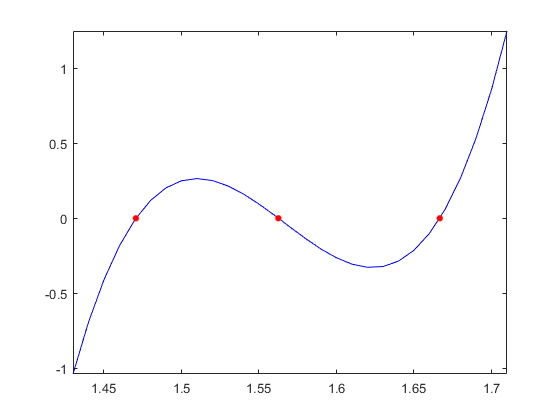
\includegraphics[width=0.6\linewidth]{px_plot}
    \centering
    \caption{The 3 roots of the polynomial $p(x)$}
    \label{px_roots}
\end{figure}

%(c) Starting with x0 = 1.5, what does Newton’s method do?
\subsection{}

Newtons method finds a zero in 11 iterations. It finds the zero at $x = \frac{25}{17}$.

Below are values of $x_i$ where $i$ is the iteration. 

\begin{minipage}{\linewidth}
\begin{lstlisting}
X_0:  1.500000000000000
X_1:  1.416666666666667
X_2:  1.450677267373387
X_3:  1.466352192549958
X_4:  1.470328933587513
X_5:  1.470587167764815
X_6:  1.470588235275914
X_7:  1.470588235294096
X_8:  1.470588235293973
X_9:  1.470588235294035
X_10: 1.470588235294158
X_11: 1.470588235294158
\end{lstlisting}
\end{minipage}

%(d) Starting with x0 = 1 and x1 = 2, what does the secant method do? 
\subsection{}

The secant method finds a zero in 12 iterations. It finds the zero at $x = \frac{5}{3}$.

Below are values of $x_i$ where $i$ is the iteration.


\begin{minipage}{\linewidth}
\begin{lstlisting}
X_0:  1.000000000000000 
X_1:  2.000000000000000 
X_2:  1.695652173913044 
X_3:  1.692189044157721 
X_4:  1.673392092119985 
X_5:  1.668509164558399 
X_6:  1.666832623252804 
X_7:  1.666671061078255 
X_8:  1.666666677366379 
X_9:  1.666666666667267 
X_10: 1.666666666666721 
X_11: 1.666666666666585 
X_12: 1.666666666666653 
X_13: 1.666666666666653 
\end{lstlisting}
\end{minipage}

%(e) Starting with the interval [1, 2], what does bisection do?
\subsection{}

The bisection method finds a zero in 52 iterations. It finds the zero at $x = \frac{25}{17}$.

Below are the upper and lower bound of the search interval in each iteration.

\begin{minipage}{\linewidth}
\begin{lstlisting}
step 0:  a = 1.000000000000000, b = 2.000000000000000
step 1:  a = 1.000000000000000, b = 1.500000000000000
step 2:  a = 1.250000000000000, b = 1.500000000000000
step 3:  a = 1.375000000000000, b = 1.500000000000000
step 4:  a = 1.437500000000000, b = 1.500000000000000
step 5:  a = 1.468750000000000, b = 1.500000000000000
step 6:  a = 1.468750000000000, b = 1.484375000000000
step 7:  a = 1.468750000000000, b = 1.476562500000000
step 8:  a = 1.468750000000000, b = 1.472656250000000
step 9:  a = 1.468750000000000, b = 1.470703125000000
step 10: a = 1.469726562500000, b = 1.470703125000000
step 11: a = 1.470214843750000, b = 1.470703125000000
step 12: a = 1.470458984375000, b = 1.470703125000000
step 13: a = 1.470581054687500, b = 1.470703125000000
step 14: a = 1.470581054687500, b = 1.470642089843750
step 15: a = 1.470581054687500, b = 1.470611572265625
step 16: a = 1.470581054687500, b = 1.470596313476563
step 17: a = 1.470581054687500, b = 1.470588684082031
step 18: a = 1.470584869384766, b = 1.470588684082031
step 19: a = 1.470586776733398, b = 1.470588684082031
step 20: a = 1.470587730407715, b = 1.470588684082031
step 21: a = 1.470588207244873, b = 1.470588684082031
step 22: a = 1.470588207244873, b = 1.470588445663452
step 23: a = 1.470588207244873, b = 1.470588326454163
step 24: a = 1.470588207244873, b = 1.470588266849518
step 25: a = 1.470588207244873, b = 1.470588237047195
step 26: a = 1.470588222146034, b = 1.470588237047195
step 27: a = 1.470588229596615, b = 1.470588237047195
step 28: a = 1.470588233321905, b = 1.470588237047195
step 29: a = 1.470588235184550, b = 1.470588237047195
step 30: a = 1.470588235184550, b = 1.470588236115873
step 31: a = 1.470588235184550, b = 1.470588235650212
step 32: a = 1.470588235184550, b = 1.470588235417381
step 33: a = 1.470588235184550, b = 1.470588235300966
step 34: a = 1.470588235242758, b = 1.470588235300966
step 35: a = 1.470588235271862, b = 1.470588235300966
step 36: a = 1.470588235286414, b = 1.470588235300966
step 37: a = 1.470588235293690, b = 1.470588235300966
step 38: a = 1.470588235293690, b = 1.470588235297328
step 39: a = 1.470588235293690, b = 1.470588235295509
step 40: a = 1.470588235293690, b = 1.470588235294599
step 41: a = 1.470588235294144, b = 1.470588235294599
step 42: a = 1.470588235294144, b = 1.470588235294372
step 43: a = 1.470588235294144, b = 1.470588235294258
step 44: a = 1.470588235294144, b = 1.470588235294201
step 45: a = 1.470588235294144, b = 1.470588235294173
step 46: a = 1.470588235294144, b = 1.470588235294159
step 47: a = 1.470588235294152, b = 1.470588235294159
step 48: a = 1.470588235294155, b = 1.470588235294159
step 49: a = 1.470588235294155, b = 1.470588235294157
step 50: a = 1.470588235294156, b = 1.470588235294157
step 51: a = 1.470588235294156, b = 1.470588235294156
step 52: a = 1.470588235294156, b = 1.470588235294156
\end{lstlisting}
\end{minipage}


%(f) What is fzerotx(p,[1,2])? Why?
\subsection{}

\textit{fzerotx} returns a value of 1.666666666666669, corresponding to the zero at $x = \frac{5}{3}$.

\textit{fzerotx} uses an improved version of the secant algorithm. It approaches 0 in a similar way as secant, following the slope from $x=2$ towards $x=1$. Thats why it it finds the zero closest to $x=2$ at $x = \frac{5}{3}$.

\textit{fzerotx} gives a slightly less accurate answer than my implementation of secant because it uses a threshold that is approximately 2 times machine epsilon.


\begin{figure}[t!]
    \begin{subfigure}[t]{0.32\textwidth}
        \centering
        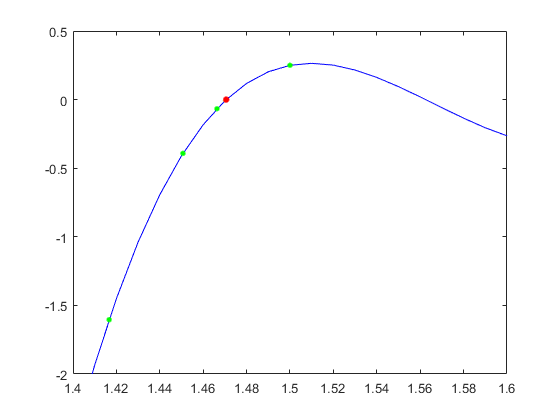
\includegraphics[width=\linewidth]{px_newton}
        \caption{Newton method}
        \label{fig_newton}
    \end{subfigure}
    \begin{subfigure}[t]{0.32\textwidth}
        \centering
        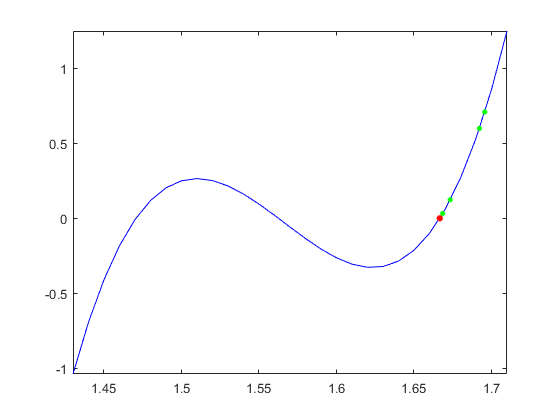
\includegraphics[width=\linewidth]{px_secant}
        \caption{Secant method}
        \label{fig_secant}
    \end{subfigure}
    \begin{subfigure}[t]{0.32\textwidth}
        \centering
        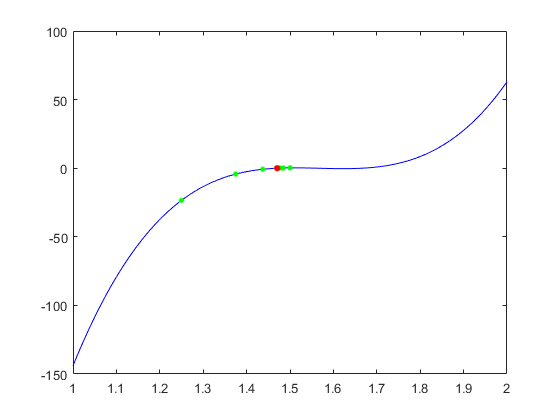
\includegraphics[width=\linewidth]{px_bisection}
        \caption{Bisection method}
        \label{fig_bisection}
    \end{subfigure}
    \caption{Points evaluated by each of the zero finding methods}
    \label{fig_zero_search}
\end{figure}

%% 4.9. 
%Find the first ten positive values of x for which x = tan x.
\section{}

To find where $x = tan(x)$ I defined the function $f(x) = x-tan(x)$ and found where that is equal to zero. $tan$ is $\pi$ periodic and continuous on the interval $[c\pi - \frac{\pi}{2}, c\pi + \frac{\pi}{2}]$ where $c$ is some whole number. Since $tan$ is only positive on the upper half of the interval, thats where I searched for zeros. I used \textit{fzero} on the interval 
$[c\pi, c\pi + \frac{\pi}{2} - \epsilon]$ for $c = 1,2, \dots,10$. $\epsilon$ is a small value I subtracted from the upper bound to avoid falling on the wrong side of the singularity and getting a value with the wrong sign.

Below are the 10 values of x that satisfy the condition $x = tan(x)$. These values accurate to within about $10^{-11}$.

\begin{minipage}{\linewidth}
\begin{lstlisting}
x = 4.493409457909064
x = 7.725251836937708
x = 10.904121659428899
x = 14.066193912831473
x = 17.220755271930770
x = 20.371302959287561
x = 23.519452498689006
x = 26.666054258812672
x = 29.811598790892958
x = 32.956389039822476
\end{lstlisting}
\end{minipage}


%% 4.16
%Utilities must avoid freezing water mains. If we assume uniform soil conditions, the temperature T(x,t) 
%at a distance x below the surface and time t after the beginning of a cold snap is given approximately by
%(T(x,t)−T_s)/(T_i-T_s) = erf(x / 2*sqrt(α*t))
%Here Ts is the constant surface temperature during the cold period, T_i is the initial soil temperature 
%before the cold snap, and α is the thermal conductivity of the soil. If x is measured in meters and t in 
%seconds, then α = 0.138 · 10−6 m2/s. Let T_i = 20◦ C, and T_s = −15◦ C, and recall that water freezes at 0◦ C. 
%Use fzerotx to determine how deep a water main should be buried so that it will not freeze until at least 
%60 days’ exposure under these conditions.
\section{}

Since every thing is given except the depth I can rewrite the formula to get the temperature as a function of depth. 
$T(x) = 35\erf(\frac{x}{2\sqrt{\alpha t}}) - 15$. We want to know at what depth is the temperature equal to zero. To find zero I used \textit{fzerotx} on the function $T$ and the interval $[0, 5]$. I picked 5 arbitrary based on my intuition.

$T(x) = 0, x = 0.946280996267692$. About 95cm.


\end{document}